\subsection{Regular Hexagon}

A regular hexagon is a polygon with six equal sides and six equal angles (each 120°). Let $s$ be the side length of the regular hexagon.

\begin{figure}[H]
    \centering
    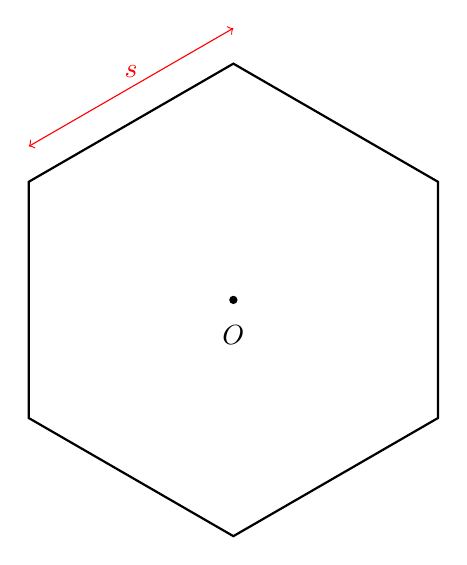
\begin{tikzpicture}[scale=1.5]
        % Draw hexagon
        \foreach \i in {0,1,2,3,4,5} {
            \coordinate (p\i) at ({90+60*\i}:2);
        }
        \draw[thick] (p0) -- (p1) -- (p2) -- (p3) -- (p4) -- (p5) -- cycle;

        % Mark one side
        \draw[<->, red] ([shift=(90:0.3)]p0) -- node[above] {$s$} ([shift=(90:0.3)]p1);

        % Draw center
        \fill (0,0) circle (1pt);
        \node at (0,-0.3) {$O$};
    \end{tikzpicture}
    \caption{Regular Hexagon with side length $s$}
\end{figure}

\textbf{Area:}
\[
    A = \frac{3\sqrt{3}}{2}s^2 \approx 2.598s^2
\]

\textbf{Diagonals:}

A regular hexagon has two types of diagonals:

\begin{figure}[H]
    \centering
    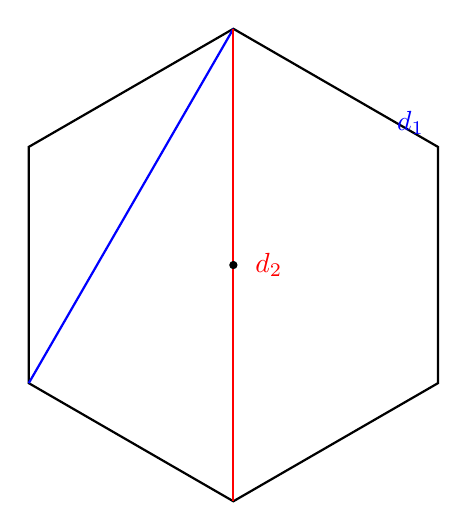
\begin{tikzpicture}[scale=1.5]
        % Draw hexagon
        \foreach \i in {0,1,2,3,4,5} {
            \coordinate (p\i) at ({90+60*\i}:2);
        }
        \draw[thick] (p0) -- (p1) -- (p2) -- (p3) -- (p4) -- (p5) -- cycle;

        % Draw short diagonal
        \draw[blue, thick] (p0) -- (p2);
        \node[blue] at (1.5,1.2) {$d_1$};

        % Draw long diagonal
        \draw[red, thick] (p0) -- (p3);
        \node[red] at (0.3,0) {$d_2$};

        % Draw center
        \fill (0,0) circle (1pt);
    \end{tikzpicture}
    \caption{Hexagon diagonals: short diagonal $d_1$ (blue) and long diagonal $d_2$ (red)}
\end{figure}

Short diagonal (connecting vertices separated by one vertex):
\[
    d_1 = \sqrt{3}s
\]

Long diagonal (connecting opposite vertices):
\[
    d_2 = 2s
\]

\textbf{Circumradius and Inradius:}

\begin{figure}[H]
    \centering
    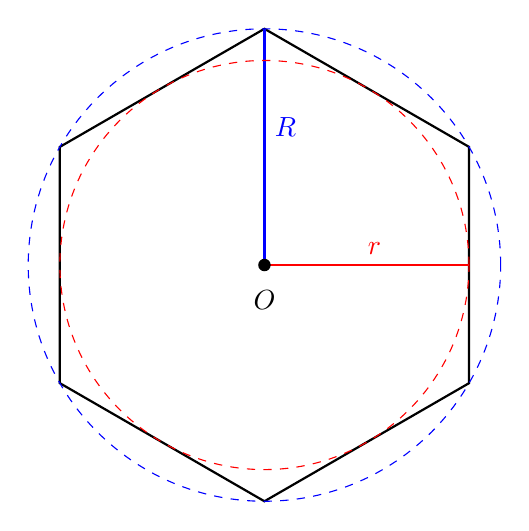
\begin{tikzpicture}[scale=1.5]
        % Draw hexagon
        \foreach \i in {0,1,2,3,4,5} {
            \coordinate (p\i) at ({90+60*\i}:2);
        }
        \draw[thick] (p0) -- (p1) -- (p2) -- (p3) -- (p4) -- (p5) -- cycle;

        % Draw circumcircle
        \draw[dashed, blue] (0,0) circle (2);
        \draw[blue, thick] (0,0) -- node[above right] {$R$} (p0);

        % Draw incircle
        \draw[dashed, red] (0,0) circle (1.732);
        \draw[red, thick] (0,0) -- node[above, shift={(0.1,0)}] {$r$} (1.732,0);

        % Draw center
        \fill (0,0) circle (1.5pt);
        \node at (0,-0.3) {$O$};
    \end{tikzpicture}
    \caption{Circumradius $R$ (blue) and inradius $r$ (red)}
\end{figure}

Circumradius (radius of circumscribed circle):
\[
    R = s
\]

Inradius (radius of inscribed circle, or apothem):
\[
    r = \frac{\sqrt{3}}{2}s \approx 0.866s
\]

Relationship between circumradius and inradius:
\[
    r = \frac{\sqrt{3}}{2}R
\]

\textbf{Area from radius:}

Area in terms of circumradius $R$:
\[
    A = \frac{3\sqrt{3}}{2}R^2
\]

Area in terms of inradius $r$:
\[
    A = 2\sqrt{3}r^2
\]

\textbf{Internal angles:}

The sum of all internal angles is $(6-2) \times 180° = 720°$

Each internal angle of a regular hexagon is $120°$
